A sailboat can achive velocity by catching wind in the sail at different angles. This is called point of sail and the velocity is dependent on the displacement from the wind direction where the velocity is a resultant of the force vector created by the wind depending on the alignemnt of the sail and the direction from where the wind is coming. A higher force and therefore also velocity is achived by sailing downwind, away from the origin of the wind. There are five different states of point of sail that are divided into degrees away from the true wind origin. These are
\begin{labeling}{alligator}
\item [Luffing] (no propulsive force) angle between 0-30\degree
\item [Close-hauled] (lift) angle between 30-50\degree
\item [Beam reach] (lift) angle 90\degree
\item [Broad reach] (lift–drag) andgle aound 135\degree
\item [Running] (drag) angle around 180\degree
\end{labeling}
and is represented in figure \ref{points-sail}. A sailor wants to prevent the sail from luffing when the sail starts to flap in the wind and no propulsive force is achived. When the 
\begin{figure}[H]
\centering
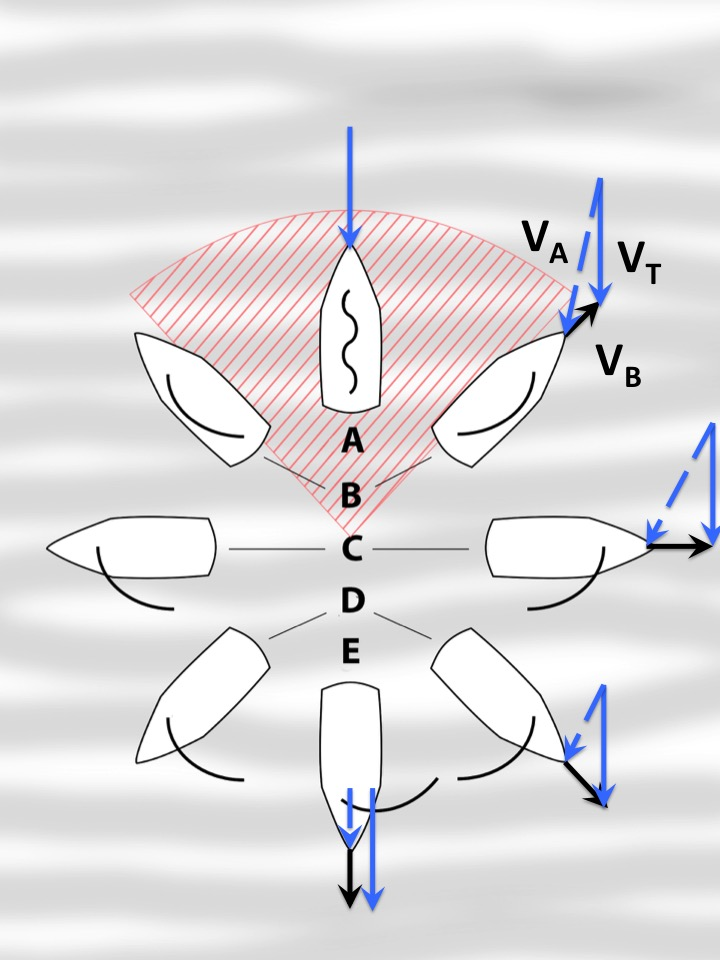
\includegraphics[width=0.6\textwidth]{Figures/Points_of_sail.jpg}
\caption{Points of sail}
\label{points-sail}
\end{figure}
